\section{Results}
\label{sec:results}

\subsection{Distillation baselines}
\label{sec:results-baselines}

\begin{table*}[t]
  \centering
  \caption{Test macro-F1 and top-1 accuracy, mean $\pm$ sample std over three seeds. Bold: best mean in a column within a student. $^{\dagger}$\Pqk with the validation-selected adaptive $\lambda$ (elsewhere $\lambda=1$). $^{\S}$One of the three seeds used a different training budget, and $^{\P}$the seeds of the \Kd cell used two different temperatures\extra{ (Appendix~\ref{app:recipe})}. \Rkd was not part of the final grid for RPS-25/LeNet-5. The primary metric is macro-F1 on TrashNet and top-1 on RPS-25.}
  \label{tab:main}
  \adjustbox{max width=\textwidth}{\begin{tabular}{@{}llcccc@{}}
\toprule
 & & \multicolumn{2}{c}{TrashNet (6 classes)} & \multicolumn{2}{c}{RPS-25 (3 classes)} \\
\cmidrule(lr){3-4}\cmidrule(lr){5-6}
Student & Method & Macro-F1 & Top-1 & Macro-F1 & Top-1 \\
\midrule
MobileNetV2-0.35 & \texttt{scratch} & $0.684\pm0.014$ & $0.697\pm0.021$ & $0.710\pm0.023$ & $0.727\pm0.030$ \\
 & \texttt{kd} & $\mathbf{0.708}\pm0.013$ & $\mathbf{0.725}\pm0.009$ & $0.710\pm0.088$ & $0.719\pm0.087$ \\
 & \texttt{rkd} & $0.672\pm0.004$ & $0.686\pm0.003$ & $\mathbf{0.737}\pm0.051$ & $\mathbf{0.745}\pm0.048$ \\
 & \texttt{rbf\_control} & $0.671\pm0.010$ & $0.692\pm0.012$ & $0.684\pm0.062$ & $0.702\pm0.059$ \\
 & \texttt{pqk} & $0.683\pm0.013$$^{\dagger}$ & $0.694\pm0.016$$^{\dagger}$ & $0.713\pm0.030$$^{\dagger}$ & $0.730\pm0.019$$^{\dagger}$ \\
\midrule
MobileNetV3-S & \texttt{scratch} & $0.724\pm0.016$ & $0.745\pm0.016$ & $0.816\pm0.053$ & $0.828\pm0.045$ \\
 & \texttt{kd} & $\mathbf{0.732}\pm0.020$ & $\mathbf{0.753}\pm0.021$ & $0.830\pm0.089$ & $0.843\pm0.075$ \\
 & \texttt{rkd} & $0.716\pm0.003$ & $0.736\pm0.007$ & $0.849\pm0.048$ & $0.859\pm0.041$ \\
 & \texttt{rbf\_control} & $0.715\pm0.037$ & $0.730\pm0.040$ & $\mathbf{0.888}\pm0.063$ & $\mathbf{0.892}\pm0.060$ \\
 & \texttt{pqk} & $0.718\pm0.009$$^{\dagger}$ & $0.735\pm0.008$$^{\dagger}$ & $0.840\pm0.065$ & $0.851\pm0.054$ \\
\midrule
LeNet-5 & \texttt{scratch} & $0.529\pm0.021$ & $0.541\pm0.022$ & $\mathbf{0.676}\pm0.108$$^{\S}$ & $\mathbf{0.676}\pm0.109$$^{\S}$ \\
 & \texttt{kd} & $0.484\pm0.074$ & $0.490\pm0.075$ & $0.650\pm0.012$$^{\P}$ & $0.652\pm0.016$$^{\P}$ \\
 & \texttt{rkd} & $\mathbf{0.578}\pm0.016$ & $\mathbf{0.597}\pm0.021$ & -- & -- \\
 & \texttt{rbf\_control} & $0.539\pm0.008$ & $0.552\pm0.007$ & $0.538\pm0.202$ & $0.584\pm0.153$ \\
 & \texttt{pqk} & $0.535\pm0.003$ & $0.552\pm0.003$ & $0.638\pm0.070$ & $0.642\pm0.058$ \\
\bottomrule
\end{tabular}
}
\end{table*}

\begin{figure*}[t]
  \centering
  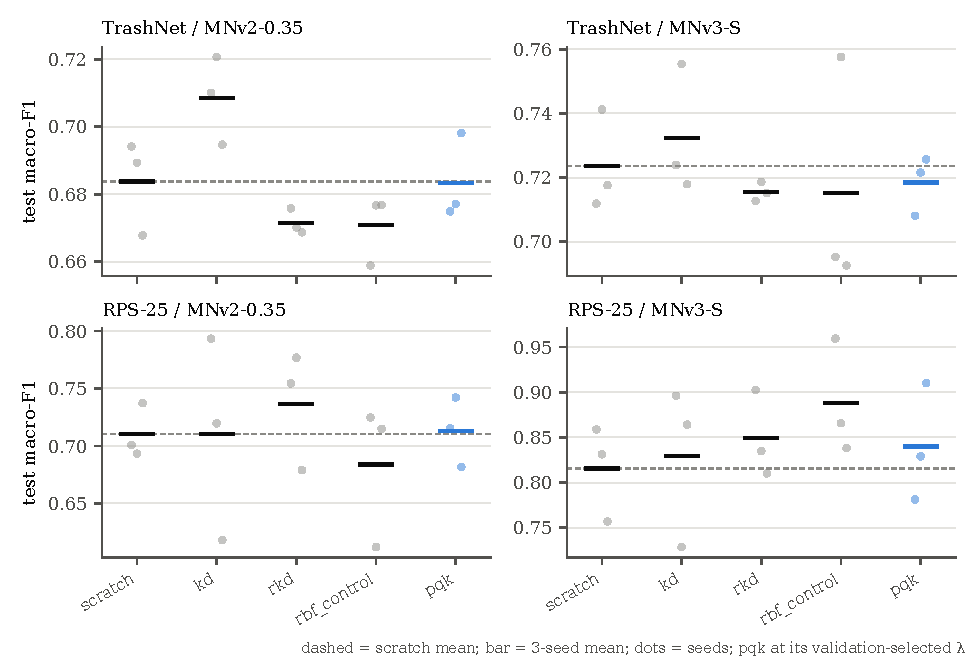
\includegraphics[width=0.95\textwidth]{methods_seeds}
  \caption{Test macro-F1 of the five methods for the four MobileNet pairs. Dots are individual seeds, bars are means, and the dashed line is the mean of \Scratch.}
  \label{fig:methods}
\end{figure*}

Table~\ref{tab:main} and Figure~\ref{fig:methods} give the baseline picture.
Distillation helps in some pairs and not in others.
\Kd beats \Scratch on TrashNet for both MobileNets, by $+0.025\pm0.008$ (MobileNetV2-0.35) and $+0.009\pm0.007$ (MobileNetV3-Small) macro-F1, ahead on all three seeds of each. On the $0.03$\,M LeNet-5 it hurts ($-0.045\pm0.093$), and \Rkd helps ($+0.049\pm0.035$, three of three seeds).
\Rkd is slightly behind \Scratch on the TrashNet MobileNets ($-0.012$ and $-0.008$).
No method dominates.
The best mean is \Kd on the TrashNet MobileNets, \Rkd on TrashNet/LeNet-5 and RPS-25/MobileNetV2-0.35, \Rbf on RPS-25/MobileNetV3-Small, and \Scratch on RPS-25/LeNet-5. \Pqk is the best method on no pair.
The classical kernel-alignment arm \Rbf beats \Scratch on the mean in only \RbfBeatsScratch{} of \NPairs{} pairs. On RPS-25/MobileNetV3-Small it does so clearly ($+0.072\pm0.034$, three of three seeds).
On TrashNet all students stay well below the teacher: the best reaches $0.732$ macro-F1 against $0.876$. On RPS-25 the best student (the RBF twin with MobileNetV3-Small, $0.888$) comes close to the teacher's $0.907$.
Seed noise is large relative to these effects, particularly on RPS-25, where the standard deviation across seeds ranges from $0.012$ to $0.202$, against $0.003$ to $0.074$ on TrashNet.

\subsection{PQK against logit KD, the RBF twin and relational KD}
\label{sec:results-pqk}

\begin{table*}[t]
  \centering
  \caption{Paired difference $\mathtt{pqk}-\mathtt{kd}$ in test macro-F1 (mean $\pm$ std of the per-seed differences, and the number of seeds on which \Pqk is ahead). \Pqk is at its validation-selected $\lambda$ at fp32 and at the exported variant at INT8; these differ only for TrashNet/MobileNetV2-0.35, where the INT8 models use $\lambda=1$ and the fp32 column adaptive $\lambda$. $^{\P}$The \Kd cell for RPS-25/LeNet-5 mixes two temperatures\extra{ (Appendix~\ref{app:recipe})}. ``PC'' uses LiteRT's builtin kernels on x86; ``Pi'' columns were measured on the Raspberry Pi, with its builtin kernels and with its default XNNPACK delegate. LeNet-5 was not exported.}
  \label{tab:pqk-kd}
  \adjustbox{max width=\textwidth}{\begin{tabular}{@{}llcccc@{}}
\toprule
 & & fp32 & \multicolumn{3}{c}{INT8} \\
\cmidrule(lr){4-6}
Dataset & Student & test macro-F1 & PC (builtin) & Pi builtin & Pi XNNPACK \\
\midrule
TrashNet & MobileNetV2-0.35 & $-0.025\pm0.025$ (1/3) & $+0.004\pm0.006$ (2/3) & $+0.004\pm0.006$ (2/3) & $-0.004\pm0.010$ (1/3) \\
TrashNet & MobileNetV3-S & $-0.014\pm0.021$ (1/3) & $-0.017\pm0.021$ (0/3) & $-0.016\pm0.016$ (0/3) & $-0.025\pm0.015$ (0/3) \\
TrashNet & LeNet-5 & $+0.051\pm0.073$ (2/3) & -- & -- & -- \\
RPS-25 & MobileNetV2-0.35 & $+0.003\pm0.073$ (2/3) & $+0.025\pm0.108$ (2/3) & $+0.025\pm0.108$ (2/3) & $+0.032\pm0.113$ (2/3) \\
RPS-25 & MobileNetV3-S & $+0.010\pm0.112$ (2/3) & $+0.016\pm0.101$ (2/3) & $+0.017\pm0.104$ (2/3) & $+0.011\pm0.115$ (2/3) \\
RPS-25 & LeNet-5 & $-0.013\pm0.059$ (2/3)$^{\P}$ & -- & -- & -- \\
\midrule
\multicolumn{2}{@{}l}{Pairs where \texttt{pqk} is ahead on the mean} & 3/6 & 3/4 & 3/4 & 2/4 \\
\bottomrule
\end{tabular}
}
\end{table*}

\begin{figure*}[t]
  \centering
  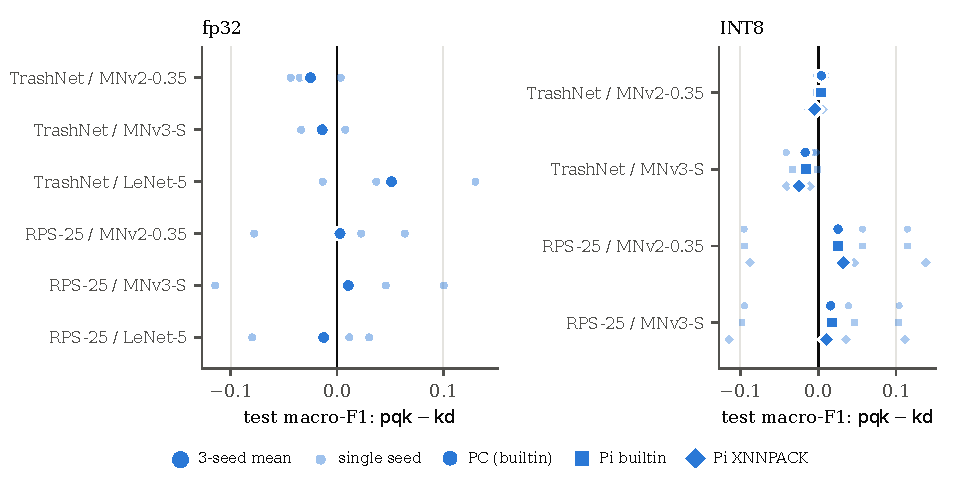
\includegraphics[width=\textwidth]{pqk_vs_kd}
  \caption{$\mathtt{pqk}-\mathtt{kd}$ per pair, paired by seed, at fp32 (left) and after INT8 conversion under three sets of kernels (right). Positive values favour \Pqk.}
  \label{fig:pqk-kd}
\end{figure*}

\paragraph{Against logit KD.}
Table~\ref{tab:pqk-kd} and Figure~\ref{fig:pqk-kd} show that \Pqk and \Kd cannot be told apart.
At fp32, \Pqk is ahead of \Kd on the mean in \KdAheadFp{} of \NPairs{} pairs. The count is \KdAheadFpEx{} if the one \Kd seed trained at a different temperature on RPS-25/LeNet-5 is excluded\extra{ (Appendix~\ref{app:recipe})}.
On TrashNet, the primary dataset, \Pqk is behind on both MobileNets, by $0.025\pm0.025$ and $0.014\pm0.021$ macro-F1, and ahead on one seed of three in each.
It is ahead on TrashNet/LeNet-5 ($+0.051\pm0.073$), where \Kd itself fails. On RPS-25 it is ahead by $+0.003\pm0.073$ (MobileNetV2-0.35) and $+0.010\pm0.112$ (MobileNetV3-Small) and behind on LeNet-5 ($-0.013\pm0.059$). On top-1, the primary metric there, the three differences are $+0.012$, $+0.008$ and $-0.010$.
After INT8 conversion, \Pqk is ahead of \Kd on the mean in \KdAheadPc{} of \NExported{} pairs on PC numerics and on the Pi's builtin kernels, and in \KdAheadXnn{} of \NExported{} on the Pi's default XNNPACK kernels.
TrashNet/MobileNetV3-Small is a loss under all three sets of kernels ($-0.017$, $-0.016$, $-0.025$, with \Pqk behind on every seed). The RPS-25 differences ($+0.011$ to $+0.032$) come with paired standard deviations of $0.10$ to $0.12$.
No difference is significant. The smallest uncorrected paired $p$-value is \MinPKd{} at fp32 and \MinPKdInt{} at INT8.
One caveat applies: the \Kd temperature was screened on some pairs, whereas the kernel methods use one untuned $\tau$ (Section~\ref{sec:setup-protocol}). This comparison is therefore not matched on that parameter.
Against \Scratch, \Pqk differs by between $-0.039$ and $+0.024$ across the six pairs, with a smallest $p$-value of \MinPScratch{}.

\begin{table*}[t]
  \centering
  \caption{Test macro-F1 of the twin \Rbf and the paired difference $\mathtt{pqk}-\mathtt{rbf\_control}$ for the two $\lambda$ calibrations of \Pqk. Adaptive $\lambda$ has only one seed on the two LeNet-5 pairs and is omitted there. $^{\S}$See Table~\ref{tab:main}.}
  \label{tab:g2}
  \adjustbox{max width=\textwidth}{\begin{tabular}{@{}llccccc@{}}
\toprule
Dataset & Student & \texttt{scratch} & \texttt{rbf\_control} & $\Delta$ \texttt{pqk} ($\lambda{=}1$) & $\Delta$ \texttt{pqk} (adaptive $\lambda$) & selected \\
\midrule
TrashNet & MobileNetV2-0.35 & $0.684\pm0.014$ & $0.671\pm0.010$ & $+0.023\pm0.016$ (3/3) & $+0.013\pm0.011$ (3/3) & adaptive \\
TrashNet & MobileNetV3-S & $0.724\pm0.016$ & $0.715\pm0.037$ & $-0.042\pm0.049$ (1/3) & $+0.003\pm0.036$ (2/3) & adaptive \\
TrashNet & LeNet-5 & $0.529\pm0.021$ & $0.539\pm0.008$ & $-0.004\pm0.010$ (2/3) & -- & $\lambda{=}1$ \\
RPS-25 & MobileNetV2-0.35 & $0.710\pm0.023$ & $0.684\pm0.062$ & $-0.028\pm0.082$ (1/3) & $+0.029\pm0.088$ (1/3) & adaptive \\
RPS-25 & MobileNetV3-S & $0.816\pm0.053$ & $0.888\pm0.063$ & $-0.048\pm0.125$ (1/3) & $-0.058\pm0.011$ (0/3) & $\lambda{=}1$ \\
RPS-25 & LeNet-5 & $0.676\pm0.108$$^{\S}$ & $0.538\pm0.202$ & $+0.100\pm0.145$ (2/3) & -- & $\lambda{=}1$ \\
\midrule
\multicolumn{5}{@{}l}{Pairs where \texttt{pqk} beats its twin on the 3-seed mean} & \multicolumn{2}{l}{2/6 ($\lambda{=}1$); 3/4 (adaptive)} \\
\bottomrule
\end{tabular}
}
\end{table*}

\begin{figure*}[t]
  \centering
  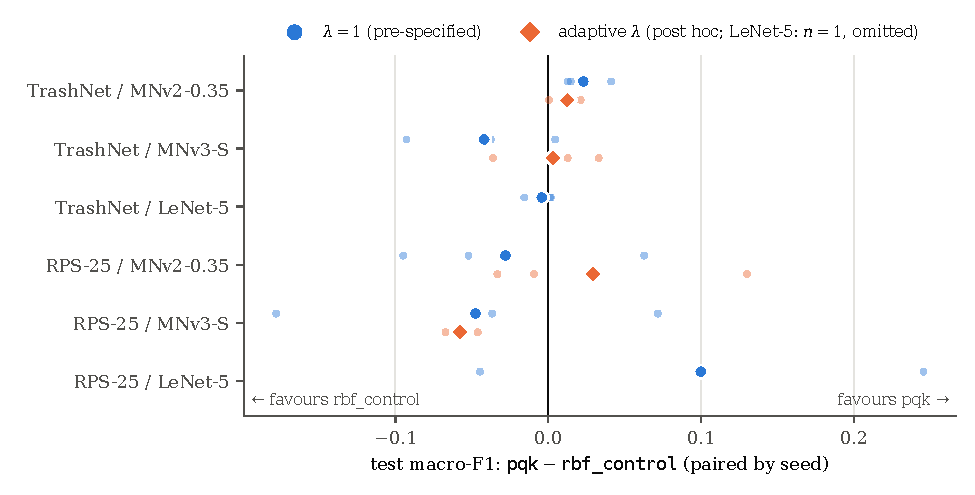
\includegraphics[width=\textwidth]{g2_paired}
  \caption{$\mathtt{pqk}-\mathtt{rbf\_control}$ per pair and seed, for the pre-specified $\lambda=1$ and for the adaptive $\lambda$ adopted after the first results. Large markers are three-seed means.}
  \label{fig:g2}
\end{figure*}

\paragraph{Against the RBF twin.}
At the pre-specified $\lambda=1$, \Pqk is ahead of its twin on the mean in only \GtwoFixedWins{} of \NPairs{} pairs (Table~\ref{tab:g2}, Figure~\ref{fig:g2}). These are TrashNet/MobileNetV2-0.35 ($+0.023\pm0.016$, three of three seeds) and RPS-25/LeNet-5 ($+0.100\pm0.145$, two of three). It is behind on the other four ($-0.042$, $-0.004$, $-0.028$, $-0.048$).
The two pairs it wins are the two that were evaluated first. Four further pairs did not reproduce them.
With the adaptive $\lambda$, which gives \Pqk the same calibration as the twin, \Pqk is ahead on \GtwoAdaptWins{} of \GtwoAdaptPairs{} pairs ($+0.013\pm0.011$, $+0.003\pm0.036$, $+0.029\pm0.088$) and behind on RPS-25/MobileNetV3-Small ($-0.058\pm0.011$). It wins on $3$, $2$, $1$ and $0$ seeds of three respectively, so the second and third winning means rest on one or two seeds.
The smallest $p$-value for $\lambda=1$ is \MinPRbfFixed{}. For the adaptive variant it is \MinPRbfAdapt{}, on RPS-25/MobileNetV3-Small, where the difference favours \MinPRbfAdaptFavours.
The quantum kernel shows no consistent advantage over its classical counterpart.

\begin{table*}[t]
  \centering
  \caption{Paired difference $\mathtt{pqk}-\mathtt{rkd}$ in test macro-F1. \Rkd was not part of the final grid for RPS-25/LeNet-5.}
  \label{tab:pqk-rkd}
  \adjustbox{max width=0.85\textwidth}{\begin{tabular}{@{}llcc@{}}
\toprule
Dataset & Student & \texttt{rkd} & $\Delta$ \texttt{pqk} $-$ \texttt{rkd} \\
\midrule
TrashNet & MobileNetV2-0.35 & $0.672\pm0.004$ & $+0.012\pm0.016$ (2/3) \\
TrashNet & MobileNetV3-S & $0.716\pm0.003$ & $+0.003\pm0.008$ (2/3) \\
TrashNet & LeNet-5 & $0.578\pm0.016$ & $-0.043\pm0.018$ (0/3) \\
RPS-25 & MobileNetV2-0.35 & $0.737\pm0.051$ & $-0.024\pm0.023$ (1/3) \\
RPS-25 & MobileNetV3-S & $0.849\pm0.048$ & $-0.009\pm0.111$ (1/3) \\
RPS-25 & LeNet-5 & -- & -- \\
\bottomrule
\end{tabular}
}
\end{table*}

\paragraph{Against relational KD.}
QRKD is a quantum extension of RKD, so \Rkd is the classical ancestor of \Pqk (Table~\ref{tab:pqk-rkd}).
\Pqk is ahead of \Rkd on the two TrashNet MobileNet pairs ($+0.012\pm0.016$ and $+0.003\pm0.008$). It is behind on TrashNet/LeNet-5 ($-0.043\pm0.018$, behind on every seed, $p=0.052$), RPS-25/MobileNetV2-0.35 ($-0.024\pm0.023$) and RPS-25/MobileNetV3-Small ($-0.009\pm0.111$).
That is \RkdAhead{} of \RkdPairs{} pairs, by at most \RkdMaxLead{} macro-F1.
The setting differs from that of QRKD, so this is not a failed replication. We do not observe consistent gains over classical relational distillation.

\subsection{Seed-to-seed variance}
\label{sec:results-variance}

\begin{table*}[t]
  \centering
  \caption{Standard deviation of test macro-F1 across the three seeds. Bold: lowest of the five methods, with \Pqk at its validation-selected $\lambda$ (last column); the two fixed and adaptive columns show both calibrations. The last row is the root mean square over pairs (adaptive: four pairs, \Rkd: five). $^{\S}$,$^{\P}$See Table~\ref{tab:main}.}
  \label{tab:var}
  \adjustbox{max width=\textwidth}{\begin{tabular}{@{}llccccccc@{}}
\toprule
Dataset & Student & \texttt{scratch} & \texttt{kd} & \texttt{rkd} & \texttt{rbf\_control} & \texttt{pqk} $\lambda{=}1$ & \texttt{pqk} adaptive & \texttt{pqk} selected \\
\midrule
TrashNet & MobileNetV2-0.35 & $0.014$ & $0.013$ & $\mathbf{0.004}$ & $0.010$ & $0.006$ & $0.013$ & $0.013$ \\
TrashNet & MobileNetV3-S & $0.016$ & $0.020$ & $\mathbf{0.003}$ & $0.037$ & $0.023$ & $0.009$ & $0.009$ \\
TrashNet & LeNet-5 & $0.021$ & $0.074$ & $0.016$ & $0.008$ & $0.003$ & -- & $\mathbf{0.003}$ \\
RPS-25 & MobileNetV2-0.35 & $\mathbf{0.023}$ & $0.088$ & $0.051$ & $0.062$ & $0.031$ & $0.030$ & $0.030$ \\
RPS-25 & MobileNetV3-S & $0.053$ & $0.089$ & $\mathbf{0.048}$ & $0.063$ & $0.065$ & $0.074$ & $0.065$ \\
RPS-25 & LeNet-5 & $0.108$$^{\S}$ & $\mathbf{0.012}$$^{\P}$ & -- & $0.202$ & $0.070$ & -- & $0.070$ \\
\midrule
Pooled std (root-mean-square over pairs) & & $0.052$ & $0.060$ & $0.032$ & $0.092$ & $0.042$ & $0.041$ & $0.041$ \\
\bottomrule
\end{tabular}
}
\end{table*}

\begin{figure*}[t]
  \centering
  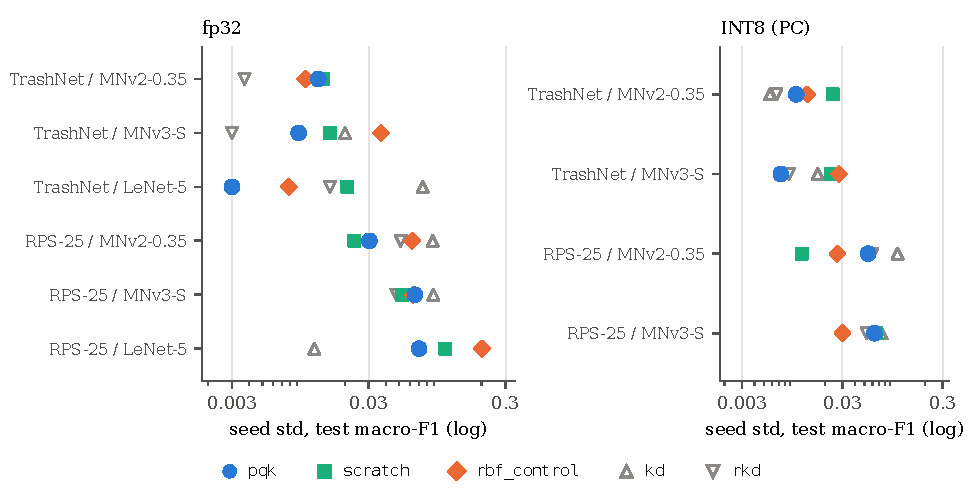
\includegraphics[width=\textwidth]{variance}
  \caption{Seed standard deviation of test macro-F1 per method and pair on a log scale, at fp32 (left) and after INT8 conversion on PC (right). \Pqk is at its validation-selected $\lambda$ at fp32 and at the exported variant at INT8.}
  \label{fig:variance}
\end{figure*}

The clearest pattern in favour of \Pqk is in the spread across seeds (Table~\ref{tab:var}, Figure~\ref{fig:variance}), and it is weaker than it first looks.
On macro-F1, with the validation-selected $\lambda$, its standard deviation is lower than that of \Rbf on \VarBelowRbf{} of \NPairs{} pairs, lower than that of \Scratch on \VarBelowScratch{}, and lower than both on three. On top-1 accuracy the counts are \VarTopBelowRbf{} and \VarTopBelowScratch{}.
Pooled over pairs (root mean square), it is \PooledPqk{} against \PooledRbf{} for \Rbf and \PooledScratch{} for \Scratch. The \Scratch figure includes the one recipe-mismatched run on RPS-25/LeNet-5\extra{ (Appendix~\ref{app:recipe})}. Without that seed the pooled \Scratch value is \PooledScratchEx{}, below that of \Pqk.
The advantage over \Rbf is the more consistent one. Against \Scratch it is fragile.
Four things limit what the pattern supports.
\emph{First}, a standard deviation from three seeds is itself very uncertain, and a sign test on four of six pairs gives $p=\SignP$.
\emph{Second}, the pattern depends on the calibration: with $\lambda=1$, \Pqk is below \Scratch on three pairs and below \Rbf on five.
\emph{Third}, it depends on the metric and on the mismatched run. Without that seed, the count against \Scratch is \VarBelowScratchEx{} of \NPairs{} on macro-F1 and \VarTopBelowScratchEx{} on top-1.
\emph{Fourth}, \Pqk is not the most stable method. On the five pairs where \Rkd exists, the pooled standard deviations are \PooledScratchFive{} for \Scratch, \PooledRkdFive{} for \Rkd and \PooledPqkFive{} for \Pqk, and \Rkd is below \Pqk on three of the five.
After INT8 conversion the pattern weakens further. Pooled over the four exported pairs on PC numerics, \Pqk has a standard deviation of \IntPooledPqk{} against \IntPooledScratch{} for \Scratch and \IntPooledRbf{} for \Rbf, because RPS-25/MobileNetV2-0.35 is noisier for \Pqk.
On TrashNet, \Pqk remains below both on both students under all three sets of kernels\extra{ (Appendix~\ref{app:int8})}.

\subsection{Entanglement and the teacher projection}
\label{sec:results-controls}

\begin{table*}[t]
  \centering
  \caption{\Pqk (adaptive $\lambda$) against the same circuit with its CNOT gates removed. Validation (decisive) and test (descriptive) macro-F1, paired by seed; $\Delta$ is $\mathtt{pqk}-\mathtt{noent\_control}$. Validation has $379$ images on TrashNet and $33$ on RPS-25.}
  \label{tab:noent}
  \adjustbox{max width=\textwidth}{\begin{tabular}{@{}llcccc@{}}
\toprule
Dataset & Student & \texttt{pqk} & no-CNOT & $\Delta$ val & $\Delta$ test \\
\midrule
TrashNet & MobileNetV2-0.35 & $0.705\pm0.006$ & $0.655\pm0.060$ & $+0.049\pm0.065$ (3/3) & $+0.059\pm0.079$ (3/3) \\
TrashNet & MobileNetV3-S & $0.737\pm0.003$ & $0.729\pm0.006$ & $+0.007\pm0.008$ (3/3) & $-0.002\pm0.028$ (1/3) \\
RPS-25 & MobileNetV2-0.35 & $0.797\pm0.083$ & $0.839\pm0.038$ & $-0.041\pm0.044$ (0/3) & $-0.060\pm0.035$ (0/3) \\
RPS-25 & MobileNetV3-S & $0.874\pm0.057$ & $0.896\pm0.037$ & $-0.022\pm0.078$ (1/3) & $-0.025\pm0.105$ (1/3) \\
\bottomrule
\end{tabular}
}
\end{table*}

\paragraph{Removing the entanglement.}
On TrashNet, whose validation split ($379$ images) is far larger than that of RPS-25, \Pqk is ahead of its entanglement-free twin on every seed of both students (validation $+0.049\pm0.065$ and $+0.007\pm0.008$, Table~\ref{tab:noent}). This is the one consistent sign that the CNOT gates contribute something beyond the sixteen trigonometric coordinates.
On RPS-25 the sign reverses ($-0.041$ and $-0.022$), on a $33$-image validation set.
Test scores point the same way except on TrashNet/MobileNetV3-Small, where the difference vanishes ($-0.002$, one seed of three).
The claim is limited.
The entanglement-free readout $(\sin4\theta,\cos4\theta)$ is highly oscillatory over $\theta\in(0,\pi)$ and may simply be a poor classical map. This result therefore does not show that \Pqk beats every classical map of equal width. The control we designed for that purpose, random Fourier features on the circuit's own frequency spectrum, was not run.
Nor did the class separation of the target kernel predict the outcome. The entanglement-free target is better aligned with the labels than the PQK target on TrashNet ($0.323$ against $0.245$ centered alignment on validation), yet students trained on the PQK target rank higher.

\begin{table*}[t]
  \centering
  \caption{Fitted minus random teacher projection, paired by seed: $\Delta$ validation and test macro-F1 for \Pqk (adaptive $\lambda$) and \Rbf. Negative values favour the random projection.}
  \label{tab:fitted}
  \adjustbox{max width=\textwidth}{\begin{tabular}{@{}llcccc@{}}
\toprule
 & & \multicolumn{2}{c}{\texttt{pqk}} & \multicolumn{2}{c}{\texttt{rbf\_control}} \\
\cmidrule(lr){3-4}\cmidrule(lr){5-6}
Dataset & Student & $\Delta$ val & $\Delta$ test & $\Delta$ val & $\Delta$ test \\
\midrule
TrashNet & MobileNetV2-0.35 & $-0.049\pm0.041$ (0/3) & $-0.060\pm0.073$ (1/3) & $-0.009\pm0.016$ (1/3) & $-0.018\pm0.003$ (0/3) \\
TrashNet & MobileNetV3-S & $-0.001\pm0.020$ (1/3) & $-0.014\pm0.019$ (1/3) & $-0.037\pm0.012$ (0/3) & $-0.013\pm0.049$ (1/3) \\
RPS-25 & MobileNetV2-0.35 & $-0.087\pm0.090$ (0/3) & $-0.104\pm0.035$ (0/3) & $-0.002\pm0.050$ (1/3) & $-0.091\pm0.125$ (1/3) \\
RPS-25 & MobileNetV3-S & $+0.043\pm0.039$ (2/3) & $+0.029\pm0.133$ (2/3) & $-0.022\pm0.036$ (0/3) & $-0.053\pm0.070$ (1/3) \\
\bottomrule
\end{tabular}
}
\end{table*}

\begin{figure*}[t]
  \centering
  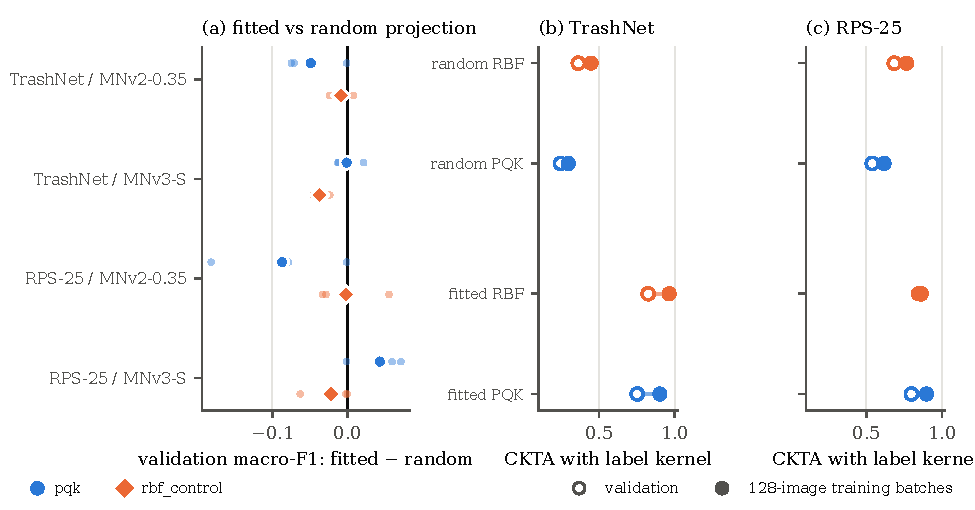
\includegraphics[width=\textwidth]{fitted_projection}
  \caption{(a)~Validation macro-F1 of a fitted (LDA+PCA) minus a random teacher projection, per seed. (b,c)~Centered kernel--target alignment (CKTA) of the target kernel the student is asked to match with the label kernel, on validation (open) and on $128$-image training batches (filled), where the loss is computed.}
  \label{fig:fitted}
\end{figure*}

\paragraph{A fitted teacher projection.}
The fixed random $2048\to8$ projection discards much of the teacher's class structure. The centered alignment of the teacher kernel with the label kernel falls from $0.720$ for the raw features to $0.363$ for the random angles on TrashNet validation.
A projection fitted on the training split (LDA+PCA) restores it ($0.825$). We selected it over PCA on validation alignment before any student was trained.
It did not help.
Fitted was better than random in \emph{one of eight} arm-pairs on validation (Table~\ref{tab:fitted}, Figure~\ref{fig:fitted}a). The exception is \Pqk on RPS-25/MobileNetV3-Small ($+0.043\pm0.039$).
The alignment measured on training batches suggests why on TrashNet.
There the fitted target is almost the label kernel on the data the loss sees: $0.963$ for the RBF target on training batches against $0.825$ on validation (random: $0.447$), and $0.902$ against $0.752$ for the PQK target (random: $0.297$ against $0.245$).
Aligning to it asks the student to cluster by class, which cross-entropy already does, and it removes the within-class geometry that relational distillation exists to transfer.
On RPS-25 the picture is mixed, and this account does not explain it. The fitted RBF target is not saturated on training batches ($0.844$ against $0.861$ on validation). The fitted PQK target is more aligned on training batches than on validation ($0.897$ against $0.797$), and that arm produced the one positive case.
The saturation account therefore covers the TrashNet results only. It is a hypothesis supported by the measurement, and we did not test it by intervention.
The measurement also shows that the selection criterion, validation alignment, was the wrong one for a relational target, because it rewards class separation.

\begin{figure*}[t]
  \centering
  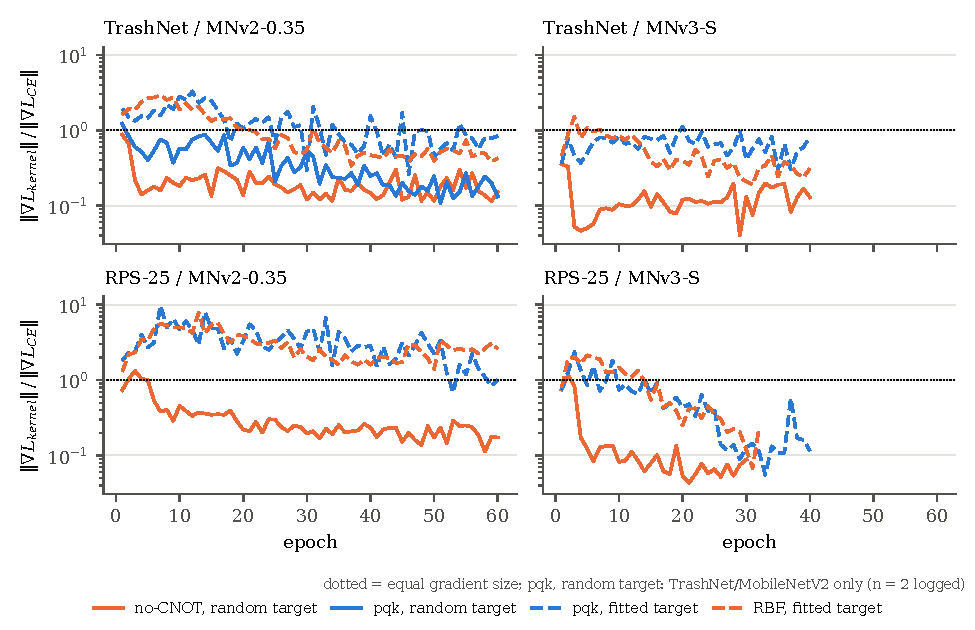
\includegraphics[width=\textwidth]{gradient_balance}
  \caption{Ratio of the gradient norm of the kernel term to that of the cross-entropy term, on the first batch of each epoch, averaged over seeds. Dashed lines use the fitted teacher projection. The solid blue line (\Pqk with a random target) was logged for TrashNet/MobileNetV2-0.35 only.}
  \label{fig:grad}
\end{figure*}

\paragraph{Does the kernel term dominate training?}
Not with the random target.
For the entanglement-free arm (12 runs), the ratio of the kernel gradient to the cross-entropy gradient falls from a mean of $0.70$ over the first three epochs to $0.14$ over the last five. For \Pqk, which was logged for only two runs (TrashNet/MobileNetV2-0.35; Figure~\ref{fig:grad}), it falls from $0.88$ to $0.20$. The label and logit terms therefore drive training after the first epochs.
With a fitted target the ratio over the last five epochs is $0.74$, $0.62$ and $0.34$ for \Pqk and $0.45$, $0.30$ and $0.28$ for \Rbf on TrashNet/MobileNetV2-0.35, TrashNet/MobileNetV3-Small and RPS-25/MobileNetV3-Small. On RPS-25/MobileNetV2-0.35 it is $3.1$ and $2.1$, and the kernel term outweighs the label signal.

\subsection{INT8 conversion}
\label{sec:results-int8}

\begin{table*}[t]
  \centering
  \caption{Change in test macro-F1 from fp32 to INT8, pooled over the exported pairs and seeds (mean, and the number of the 12 models whose score rose), for each method and set of kernels.}
  \label{tab:int8-delta}
  \adjustbox{max width=0.85\textwidth}{\begin{tabular}{@{}lccc@{}}
\toprule
Method & PC (builtin) & Pi builtin & Pi XNNPACK \\
\midrule
\texttt{scratch} & $+0.0058$ (7/12) & $+0.0038$ (7/12) & $+0.0011$ (5/12) \\
\texttt{kd} & $-0.0031$ (5/12) & $-0.0027$ (5/12) & $-0.0049$ (4/12) \\
\texttt{rkd} & $+0.0030$ (6/12) & $+0.0033$ (6/12) & $-0.0011$ (5/12) \\
\texttt{rbf\_control} & $-0.0064$ (5/12) & $-0.0045$ (5/12) & $+0.0006$ (6/12) \\
\texttt{pqk} & $+0.0080$ (9/12) & $+0.0088$ (9/12) & $+0.0025$ (5/12) \\
\bottomrule
\end{tabular}
}
\end{table*}

\begin{figure*}[t]
  \centering
  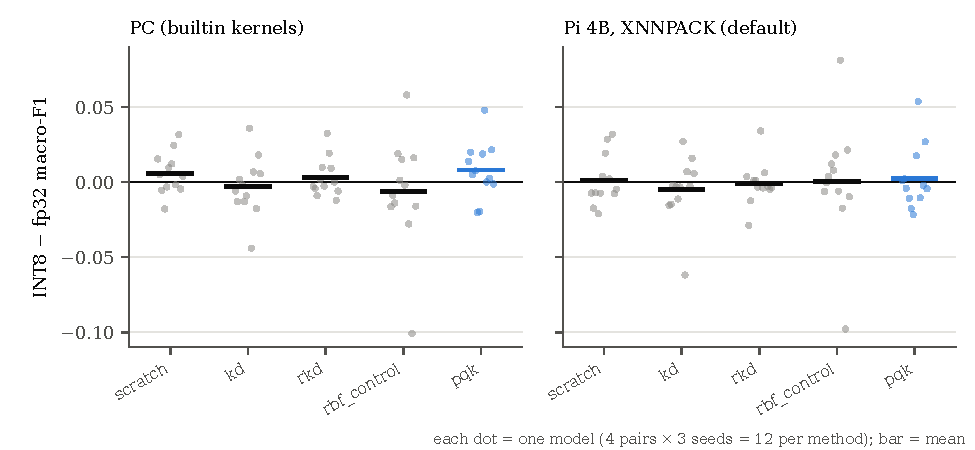
\includegraphics[width=\textwidth]{int8_delta}
  \caption{INT8 minus fp32 test macro-F1 for every exported model, by method, on PC and with the Pi's default kernels. Each dot is one model; bars are means.}
  \label{fig:int8}
\end{figure*}

All \NIntModels{} exported models pass every check. They are fully integer, quantized per channel on every convolution, contain no custom or floating-point operations, and reproduce their fp32 score exactly on reload. Their ONNX graphs match the PyTorch logits to within $1.3\times10^{-4}$\extra{ (Appendix~\ref{app:export})}.
Their size is set by the architecture alone: \MbMnvTwo{}\,MB ($604$--$608$\,KiB) for MobileNetV2-0.35 and \MbMnvThree{}\,MB ($1179$--$1181$\,KiB) for MobileNetV3-Small. Any comparison at matched size therefore holds by construction.
Conversion has no systematic cost. The macro-F1 changes by $\IntDeltaMean\pm\IntDeltaStd$ across the \NIntModels{} models, and \IntGained{} of them improve.
Conversion does change predictions. The INT8 and fp32 models disagree on about $7\%$ of test images ($91.5\%$ agreement for MobileNetV2-0.35 and $95.3\%$ for MobileNetV3-Small), in both directions.
INT8 rankings between methods are therefore fp32 rankings plus noise.
\Pqk has the most favourable change of the five methods on PC numerics ($+0.0080$, up on $9$ of $12$ models, against $-0.0031$ and $5$ of $12$ for \Kd). The difference between the two changes is not significant ($p=\QuantPPc{}$ on PC, \QuantPBuiltin{} on the Pi's builtin kernels, \QuantPXnn{} with XNNPACK), and it shrinks to $+0.0025$ with the Pi's default kernels (Table~\ref{tab:int8-delta}, Figure~\ref{fig:int8}).
The sign of other methods' changes also depends on the kernels: \Rbf moves from $-0.0064$ on PC to $+0.0006$ with XNNPACK, and \Rkd from $+0.0030$ to $-0.0011$.

\subsection{On-device behaviour}
\label{sec:results-device}

\begin{table*}[t]
  \centering
  \caption{INT8 models on the Raspberry Pi 4B with the default XNNPACK delegate, four threads, batch size 1: median (p50) and 95th-percentile (p95) invocation time over $500$ calls, mean throughput, and the speed-up from one to four threads. Latency, throughput and memory are averages over the methods and seeds of each pair (15--18 models); the thread speed-up is measured on one model per pair (\Pqk, seed~0). The spread of the p50 between methods is at most $0.11$\,ms within a pair. Sizes are in KiB.}
  \label{tab:edge}
  \adjustbox{max width=\textwidth}{\begin{tabular}{@{}llrrrrrrr@{}}
\toprule
Dataset & Student & Params & INT8 KiB & MMACs & p50 ms & p95 ms & FPS & $1\!\to\!4$ thr. \\
\midrule
TrashNet & MobileNetV2-0.35 & 403{,}814 & 608 & 18.9 & 2.53 & 2.71 & 395 & $1.84\times$ \\
TrashNet & MobileNetV3-S & 930{,}470 & 1181 & 18.2 & 3.18 & 3.35 & 314 & $1.35\times$ \\
RPS-25 & MobileNetV2-0.35 & 399{,}971 & 604 & 18.9 & 2.52 & 2.73 & 395 & $1.75\times$ \\
RPS-25 & MobileNetV3-S & 928{,}739 & 1179 & 18.2 & 3.14 & 3.30 & 318 & $1.40\times$ \\
\bottomrule
\end{tabular}
}
\end{table*}

\begin{figure*}[t]
  \centering
  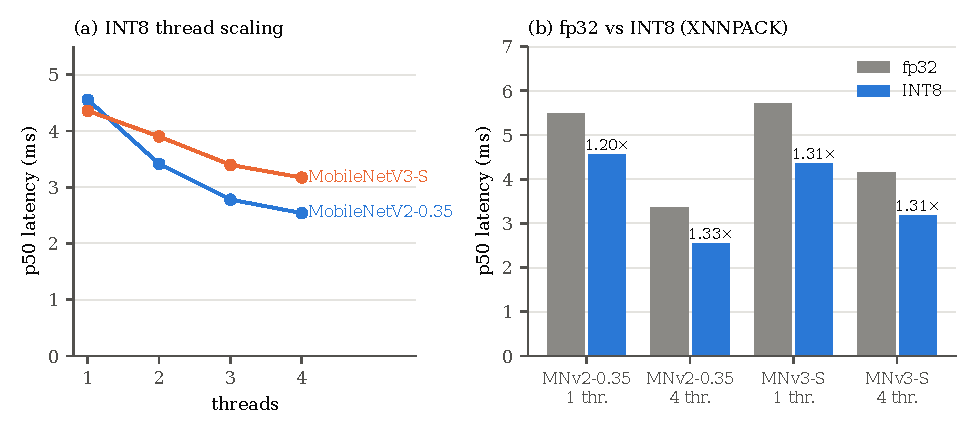
\includegraphics[width=\textwidth]{latency}
  \caption{(a)~Median INT8 latency against the number of threads. (b)~fp32 and INT8 latency with the same runtime, one and four threads, with the INT8 speed-up.}
  \label{fig:latency}
\end{figure*}

Table~\ref{tab:edge} and Figure~\ref{fig:latency} summarize the measurements ($160$ runs, none failed).
With four threads the median INT8 latency is $2.5$\,ms for MobileNetV2-0.35 and $3.2$\,ms for MobileNetV3-Small, about $395$ and $315$ inferences per second.
Latency is a property of the architecture. Within a pair, the spread between methods, which share one graph, is at most $0.11$\,ms.
The two networks do about the same work ($18.9$ and $18.2$\,M multiply--accumulates), yet MobileNetV2 is about $25\%$ faster on four threads, so operation counts do not predict speed. MobileNetV2 also scales better with threads ($1.75$--$1.84\times$ from one to four, against $1.35$--$1.40\times$), and on one thread the order reverses ($4.56$ against $4.35$\,ms on TrashNet).
Against fp32 with the same runtime (one model per pair), INT8 is $1.2$ to $1.4\times$ faster, $2.6$ to $3.1\times$ smaller, and uses less memory ($5.4$--$6.7$\,MB of interpreter memory against $8$--$12$\,MB). The speed-up is modest, and the Cortex-A72's lack of integer dot-product instructions is a likely reason.
XNNPACK is $1.1$ to $1.4\times$ faster than the builtin kernels at four threads, but it changes the model's predictions. Per model it disagrees with the PC's INT8 predictions on \XnnDisMin{}\% to \XnnDisMax{}\% of test images (\XnnDisMean{}\% on average), against at most \BuiltinDisMax{}\% (\BuiltinDisMean{}\% on average) for the builtin kernels.
It moves per-method macro-F1 by between \XnnVsPcMin{} and \XnnVsPcMax{} relative to the PC. It is also the reason the \Pqk--\Kd comparison on TrashNet/MobileNetV2-0.35 changes sign on the device ($+0.004$ on PC, $-0.004$ with XNNPACK; Table~\ref{tab:pqk-kd}).
INT8 results should therefore be reported together with the runtime that produced them.
The SoC reached at most $64.8\,^\circ$C, well below the $80\,^\circ$C throttling point. The firmware did flag an under-voltage event and a throttling event in $2$ of the $160$ runs, both at four threads, so the supply used here is marginal, and we did not attempt an energy measurement.
A live-camera pipeline\extra{ (Appendix~\ref{app:camera})} reaches about $30$ frames per second, the webcam's rate, with two inference and two OpenCV threads at $12.8$\,ms of processing per frame. Image preparation ($8.8$\,ms) costs more than inference ($4.1$\,ms). The $2.5$ and $3.2$\,ms above are invocation times only; the quantize--invoke--dequantize pipeline takes $3.4$ to $4.1$\,ms.

\subsection{Training cost}
\label{sec:results-cost}

\begin{table*}[t]
  \centering
  \caption{Compute-hours of the runs behind the reported results. Runs shared the GPU, so these are compute-hours consumed, not elapsed time, and per-epoch times are not comparable between methods. \Pqk-family hours include the CNN and the teacher forward pass, so they upper-bound the time spent simulating the circuit. Teacher fine-tuning is not included.}
  \label{tab:cost}
  \adjustbox{max width=0.9\textwidth}{\begin{tabular}{@{}lrr@{}}
\toprule
Run family & Runs kept & Compute-hours \\
\midrule
Classical (\texttt{scratch}, \texttt{kd}, \texttt{rkd}, \texttt{rbf\_control}, controls) & 98 & 49.8 \\
\texttt{pqk} family (circuit simulator in the forward pass) & 54 & 44.7 \\
\midrule
Discarded re-runs after pipeline fixes & -- & 23.0 \\
\bottomrule
\end{tabular}
}
\end{table*}

The $152$ student runs account for \CostKeptHours{} compute-hours. Of these, \CostPqkHours{} belong to the \CostPqkRuns{} runs of the \Pqk family, and a further \CostDiscardedHours{} hours went into runs discarded after pipeline fixes (Table~\ref{tab:cost}).
Because runs shared the GPU, we cannot give a clean cost ratio between methods.
The accounting does show that the circuit adds simulation to every training step of a \Pqk run, while nothing of it remains at deployment, where all methods give models of identical size and speed.
